\section{Common errors}
\label{sec:Common errors}

\subsection{Install Qt}
Inviwo uses the graphics library Qt which isn't always installed properly. These instructions show how to download and install the latest version of Qt on Ubuntu 10.04 LTS. That is, in the moment of writing this user guide, version 5.12.3. 

To download the installation file into the \emph{~/Downloads} directory, simply execute the commands below.

\begin{lstlisting}[frame = single, breaklines=true]
    cd ~/Downloads
    wget http://download.qt.io/official_releases/qt/5.12/5.12.3/qt-opensource-linux-x64-5.12.3.run
\end{lstlisting}

When the installation file has finished downloading, the user won't have permission to run the file. To change permissions and run the file by executing the commands below and enter your superuser password immediately after.
\begin{lstlisting}[frame = single, breaklines=true]
    chmod +x qt-opensource-linux-x64-5.12.3.run
    sudo ./qt-opensource-linux-x64-5.12.3.run
\end{lstlisting}

An Qt installer is now shown on the screen. Notice that the manual installation will force a installation of the Qt editor as shown in step 6. The entire installation will occupy approximately 5.12 GB. Follow the instructions in figure \ref{fig:Qt} to complete the installation.

After the installation is done, the path to Qt needs to be added to the system. Add the necessary paths by executing the commands below.

\begin{lstlisting}[frame = single, breaklines=true]
    cd /usr/lib/x86_64-linux-gnu/qtchooser
    sudo echo "/opt/Qt5.12.3/5.12.3/gcc_64/bin" | sudo tee -a default.conf
    sudo echo "/opt/Qt5.12.3/5.12.3/gcc_64/lib" | sudo tee -a default.conf
\end{lstlisting}

The system is now ready for an Inviwo installation.

\begin{figure}[H]
    \centering
    \begin{subfigure}{0.32\linewidth}
        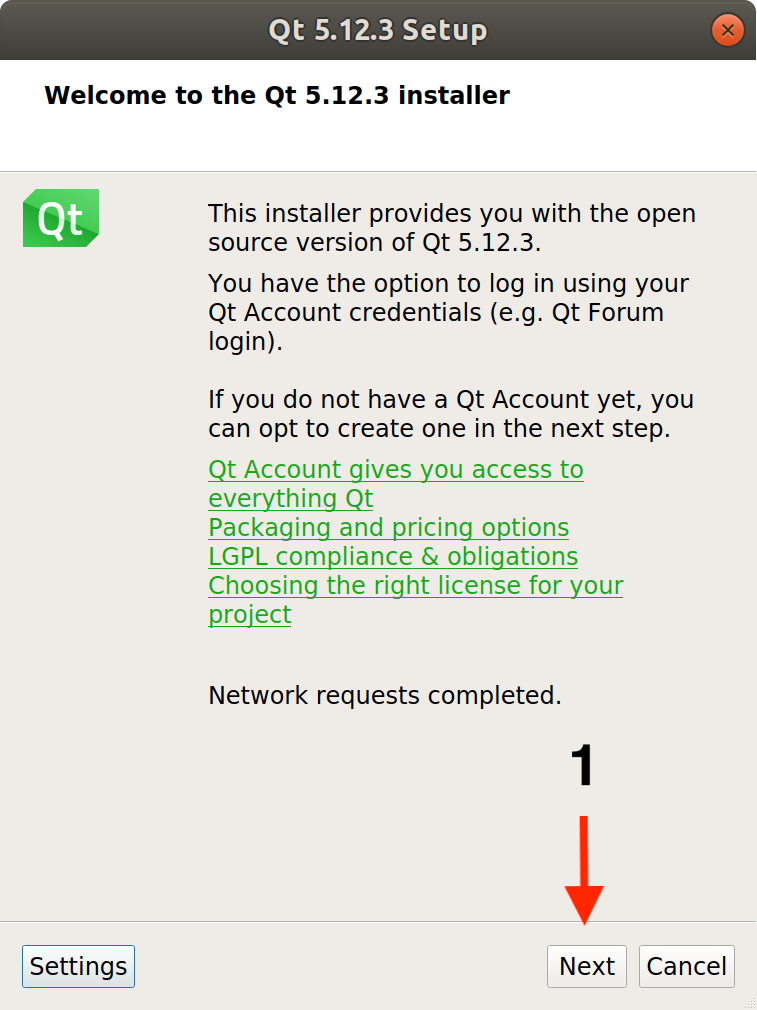
\includegraphics[width=1\textwidth]{images/Qt1.png}
    \end{subfigure}
    \begin{subfigure}{0.32\linewidth}
        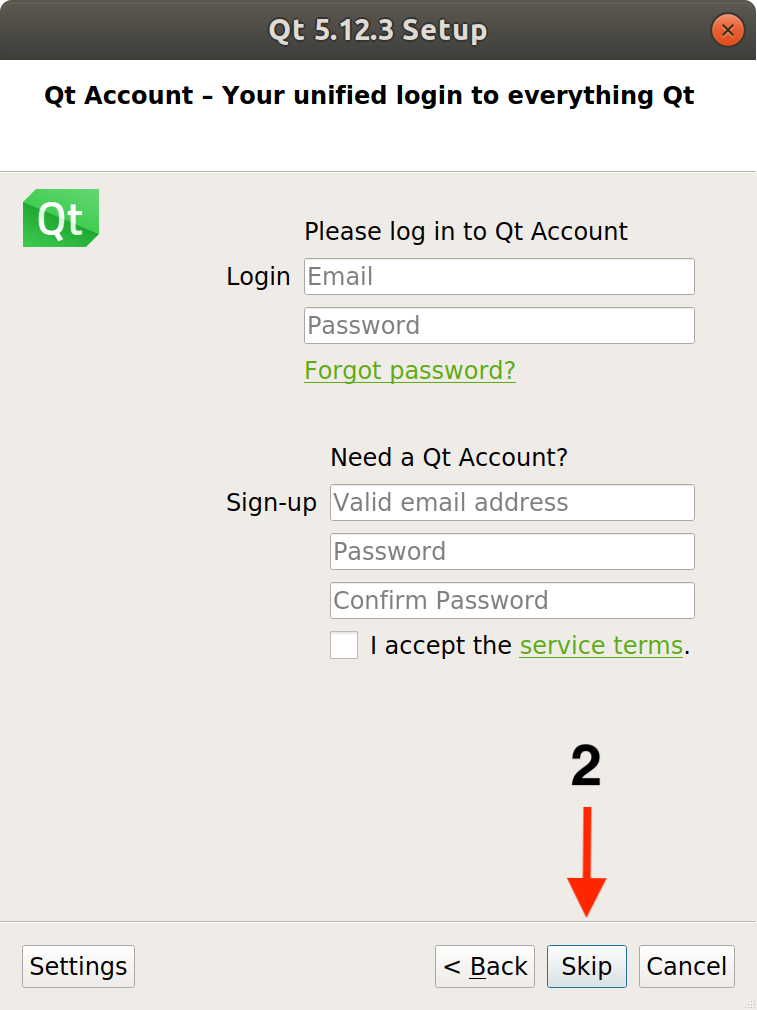
\includegraphics[width=1\textwidth]{images/Qt2.png}
    \end{subfigure}
    \begin{subfigure}{0.32\linewidth}
        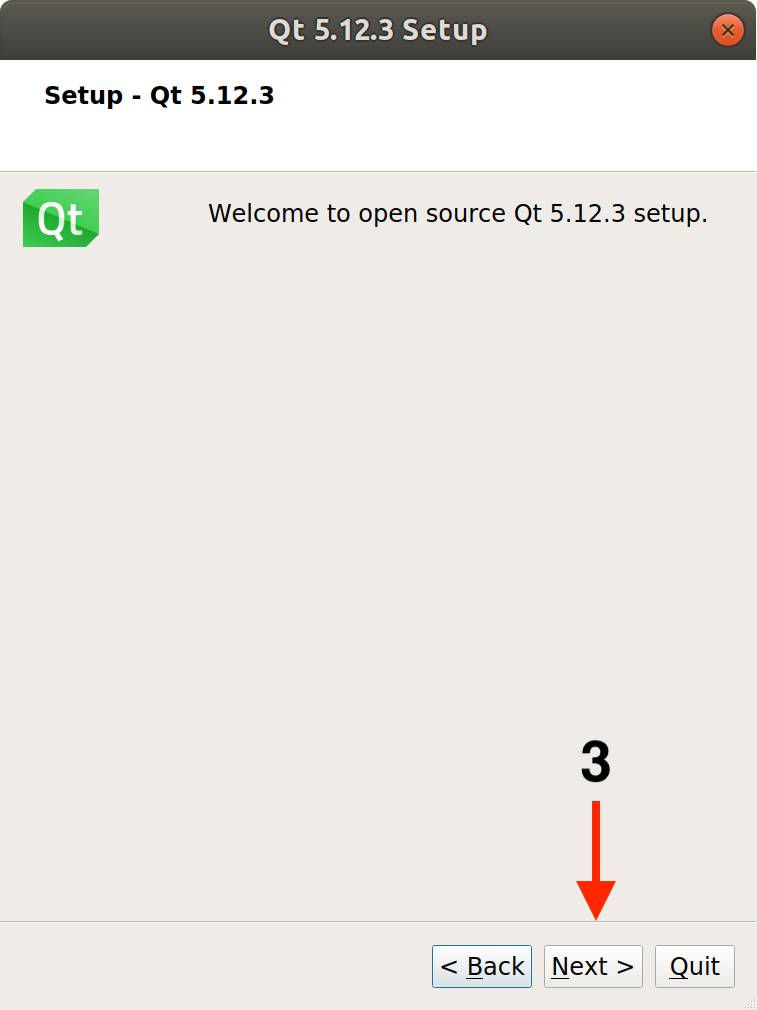
\includegraphics[width=1\textwidth]{images/Qt3.png}
    \end{subfigure}
    \begin{subfigure}{0.32\linewidth}
        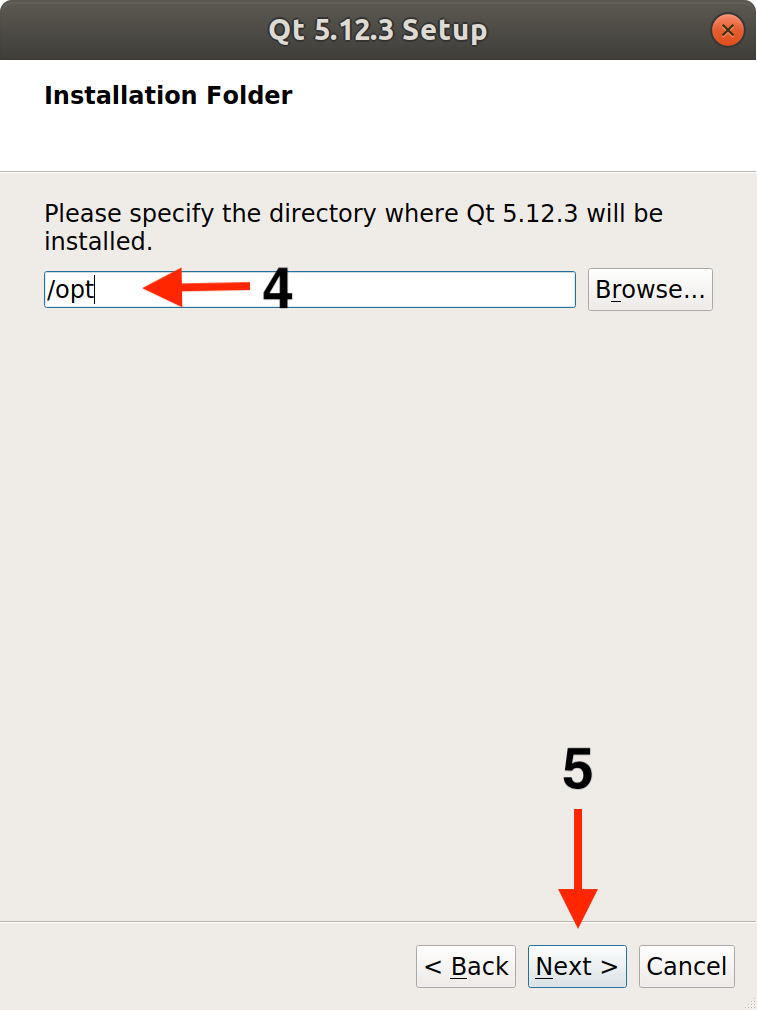
\includegraphics[width=1\textwidth]{images/Qt4.png}
    \end{subfigure}
    \begin{subfigure}{0.32\linewidth}
        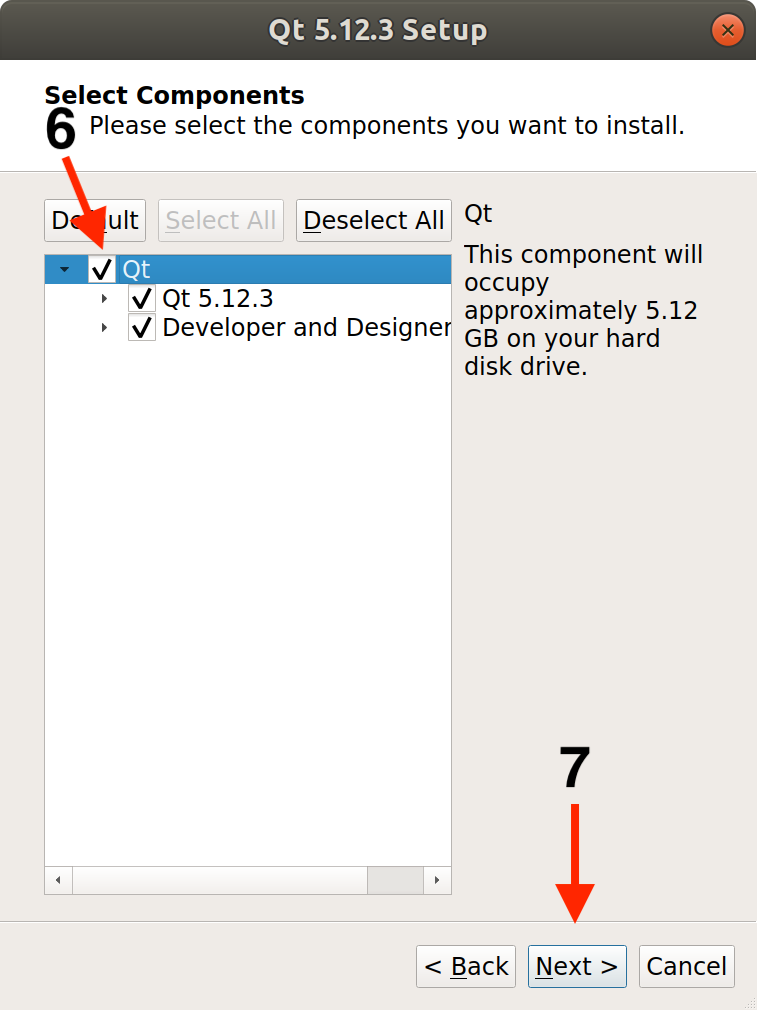
\includegraphics[width=1\textwidth]{images/Qt6.png}
    \end{subfigure}
    \begin{subfigure}{0.32\linewidth}
        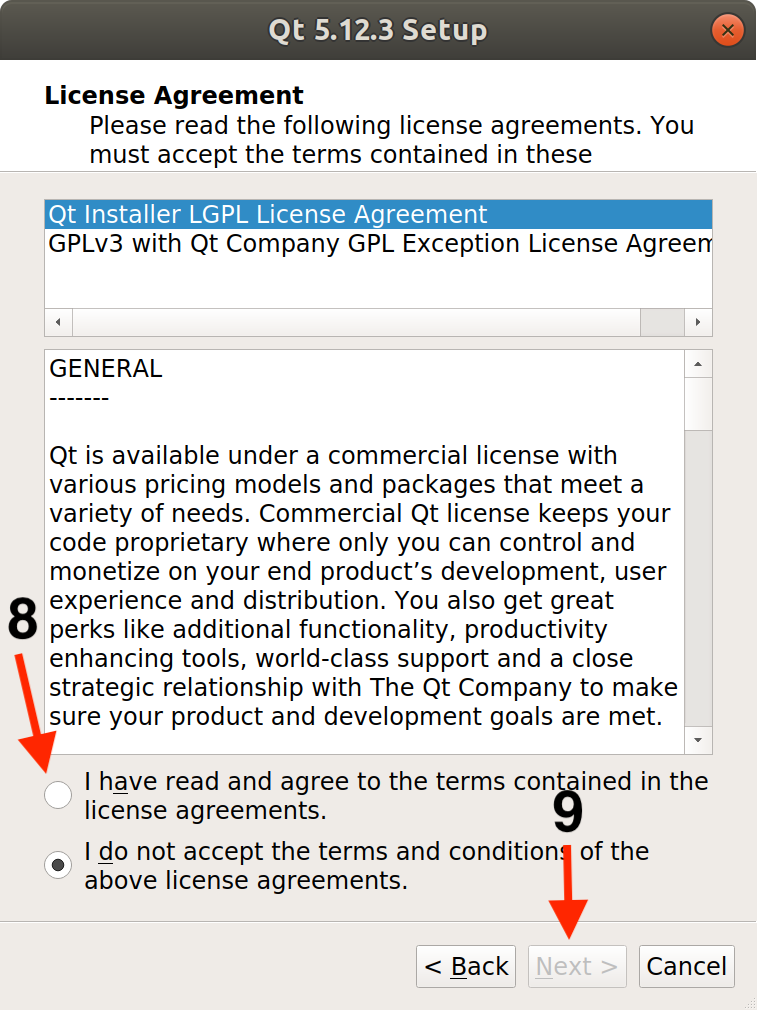
\includegraphics[width=1\textwidth]{images/Qt7.png}
    \end{subfigure}
    \begin{subfigure}{0.32\linewidth}
        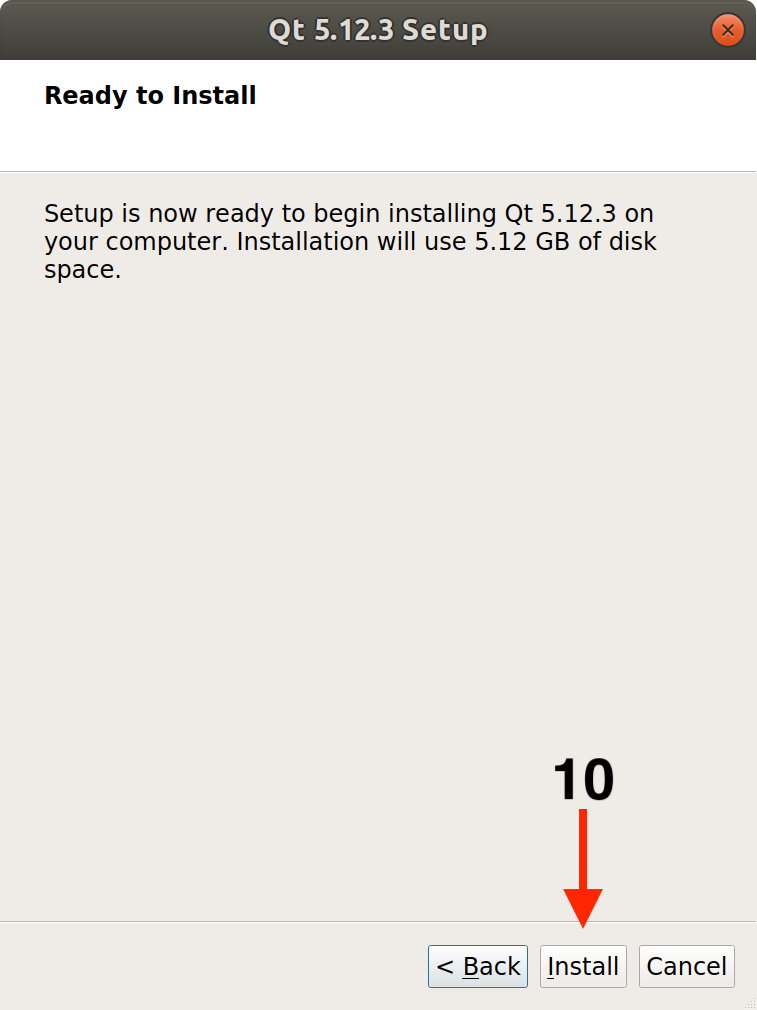
\includegraphics[width=1\textwidth]{images/Qt8.png}
    \end{subfigure}
    \caption{Instructions for installation of Qt 5.12.3.}
    \label{fig:Qt}
\end{figure}

\subsection{Set the INVIWO\_HOME path}
Before using ENVISIoN's GUI it is good to check that your environmental variable INVIWO\_HOME is set to the correct value. Otherwise the system will not find the modules inviwopy or inviwopyapp. If you have started to use the GUI you will receive the following message if the variable is not set:
\newline 
``Module error: No module named '[The missing module]'. Can not find module. Please check that the environment variable INVIWO\_HOME is set to the correct value in the computers system settings.''
\newline


\subsection{The module Inviwopyapp did not build}

If the inviwopyapp did not build when building in Visual Studio, open the project once again in Visual Studio 2017 and make sure ``inviwopyapp'' is listed to the right in the ``Solution Explorer'', see figure \ref{fig:VisStudioInviwopyapp}. Inviwopyapp should be under ``minimals'' in the list.

\begin{figure}[H]
    \centering
    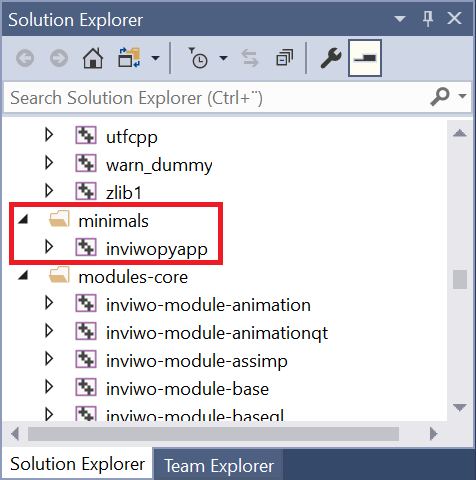
\includegraphics[scale = 0.6]{images/VisualStudioinviwopyapp.png}
    \caption{The ``Solution Explorer'' in Visual Stuido 2017}
    \label{fig:VisStudioInviwopyapp}
\end{figure}

Now try to build the project again but by choosing ``Build'' in the upper menu and then ``Build Solution'' instead of pressing fn + f5. The build should start, keep track of possible errors during the building. When it's finished, check that inviwopyapp had built.
